\documentclass[conference]{IEEEtran}
% cSpell:words Psycopg dropoff MAPE joblib checkpointing checkpointed bursty backtesting productionization geospatial Guestrin

\usepackage[utf8]{inputenc}
\usepackage[T1]{fontenc}
\usepackage{graphicx}
\usepackage{booktabs}
\usepackage{hyperref}
\usepackage{amsmath}
\usepackage{cite}
\usepackage{enumitem}
\usepackage{microtype}

\title{StreamCab: Real-Time Taxi Fare Intelligence with Kafka, Spark, and XGBoost}
\author{%
\IEEEauthorblockN{Bibek Dhungana, Xiaodi Shao, Raivath Mallela}
\IEEEauthorblockA{Big Data Application}
}
\date{\today}

\begin{document}
\maketitle

\begin{abstract}
This paper presents StreamCab, an end-to-end data engineering and machine learning system for real-time taxi analytics and short-term fare prediction. The pipeline replays historical New York City taxi trips into Apache Kafka, processes and aggregates the stream using Apache Spark Structured Streaming, stores results in PostgreSQL, and serves predictions through a dashboard interface. We describe the architecture, data processing methodology, model training strategy, and performance outcomes, then discuss practical lessons learned about reliability, memory constraints, and deployment trade-offs in single-node environments.
\end{abstract}

\section{Introduction}
Urban transportation data is high-volume, time-sensitive, and geographically heterogeneous. Static batch reports are often insufficient for operational decisions such as where demand is increasing and what pricing behavior to expect in the next few minutes. This project investigates whether a compact local stack can deliver near real-time analytics and prediction from historical taxi records replayed as live events.

The objectives of StreamCab are:
\begin{itemize}[leftmargin=1.5em]
    \item Build a reproducible streaming pipeline from data ingestion to visualization.
    \item Produce interpretable zone-level aggregate metrics over short windows.
    \item Train and serve a practical fare predictor under memory constraints.
    \item Evaluate model quality against a baseline and report engineering trade-offs.
\end{itemize}

\section{Related Work and Background}
Streaming architectures commonly use Kafka for event transport, Spark Structured Streaming for stateful transformations, and SQL databases for serving curated outputs~\cite{kafka,spark}. Gradient-boosted trees, especially XGBoost, are widely used for tabular prediction due to strong accuracy-speed trade-offs~\cite{xgboost}.

Compared to distributed cloud deployments, this project emphasizes local reproducibility and careful memory-aware design. The training pipeline uses batched parquet processing and continued model updates to support large datasets on limited RAM\@.
\section{System Architecture and Design}
\subsection{Architecture Overview}
The system has six services: PostgreSQL, Kafka (+ producer), Spark/predictor/dashboard app container, consumer, one-shot trainer, and Kafka Control Center.

\begin{figure}[!t]
    \centering
    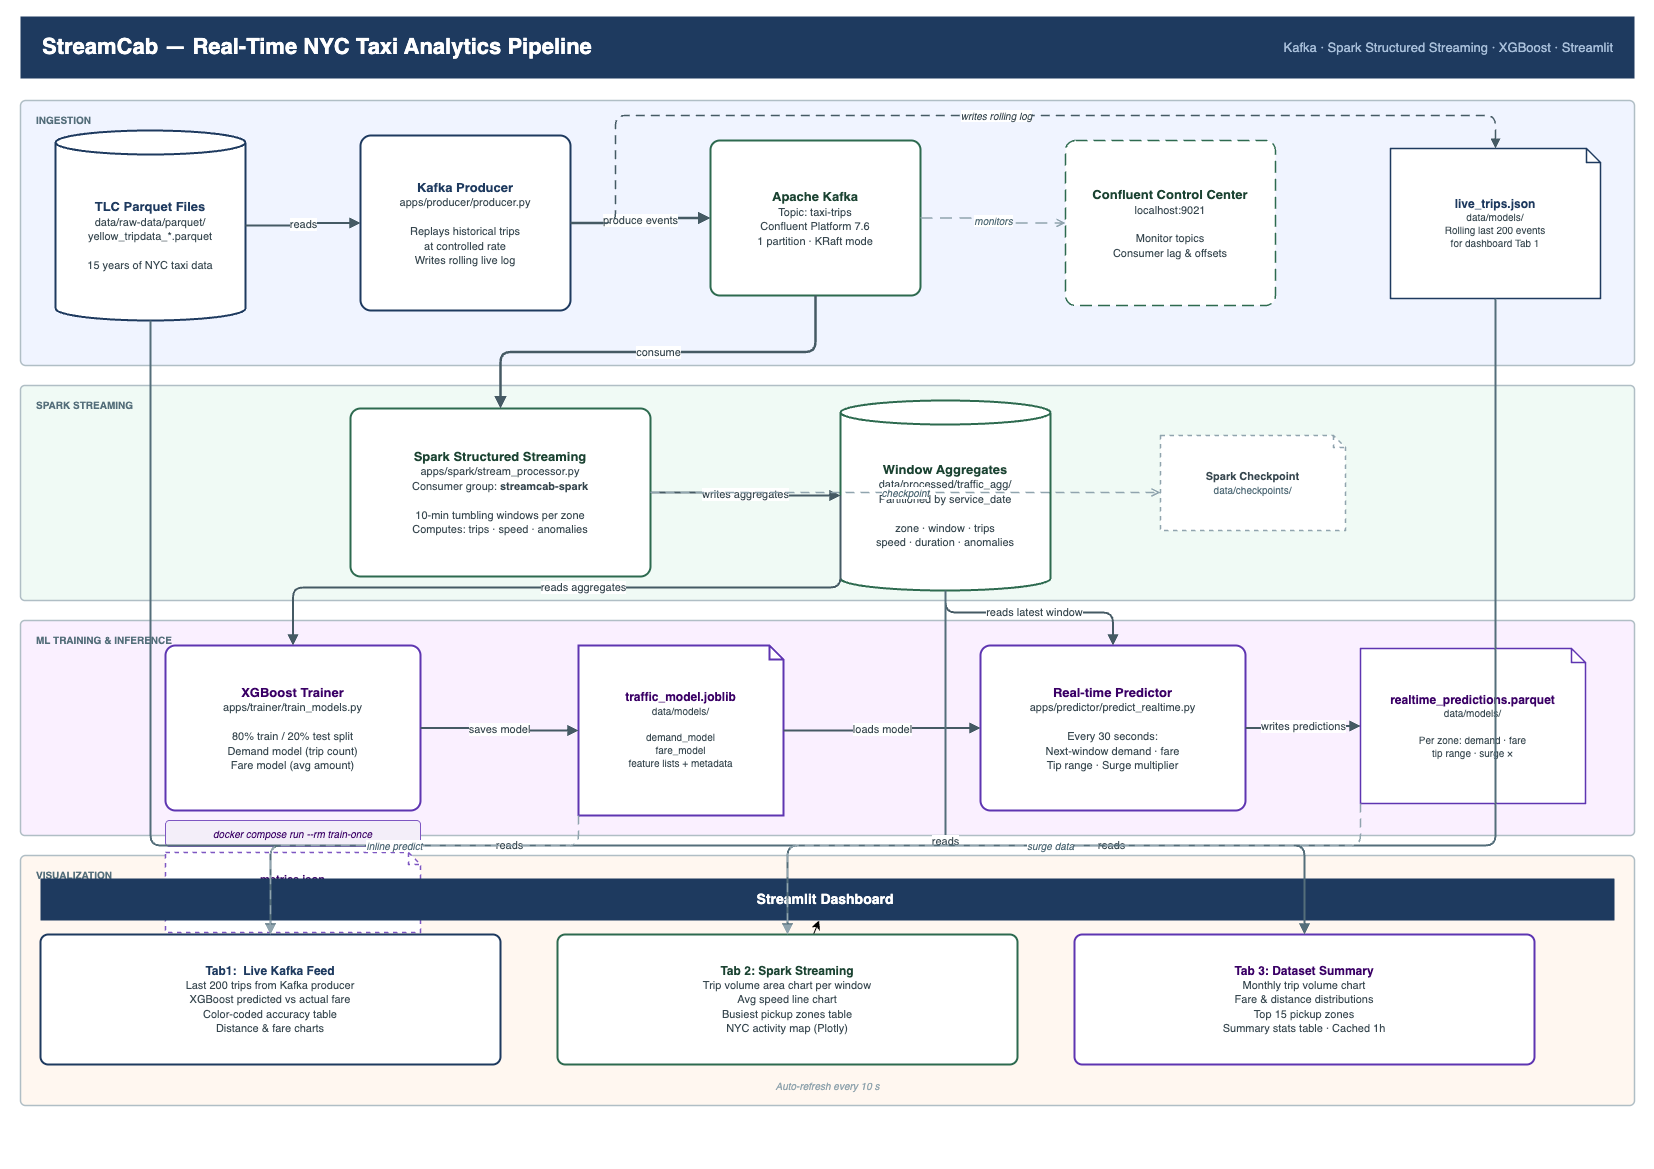
\includegraphics[width=0.95\linewidth]{../assets/architecture.png}
    \caption{StreamCab end-to-end architecture.}\label{fig:architecture}
\end{figure}

\subsection{Component Responsibilities}
\begin{itemize}[leftmargin=1.5em]
    \item \textbf{Producer:} Streams normalized trip events from parquet in replay loops.
    \item \textbf{Kafka:} Buffers and distributes trip events to downstream consumers.
    \item \textbf{Spark Structured Streaming:} Applies cleaning rules and windowed zone aggregations.
    \item \textbf{PostgreSQL:} Stores live trips, traffic aggregates, and prediction outputs.
    \item \textbf{Trainer:} Builds XGBoost fare model from historical aggregates.
    \item \textbf{Predictor + Dashboard:} Performs periodic inference and displays live analytics.
\end{itemize}

\section{Data Collection and Processing}
\subsection{Data Source}
Primary data comes from publicly available NYC TLC yellow taxi trip records (monthly parquet files).

\textbf{Data source link:} \href{https://www.nyc.gov/site/tlc/about/tlc-trip-record-data.page}{NYC TLC Trip Record Data}~\cite{tlc}

\subsection{Dataset Profile Used in This Project}
The data download utility supports monthly yellow taxi parquet files from 2010 to 2025, with a default pull range of \texttt{2022{-}01} through \texttt{2024{-}12}. For the quick-start workflow documented in the repository, a smaller slice (for example \texttt{2022{-}01} to \texttt{2022{-}03}) is used for rapid iteration and reproducible local runs.

At ingestion time, the pipeline reads only required columns (timestamps, distance, fare/amount, and zone/location fields) and applies consistency filters before aggregation. Rows are retained when duration, distance, speed, and amount fall within physically reasonable ranges, reducing outlier influence and malformed-record noise. For files that do not include pickup zone IDs, pickup latitude/longitude is snapped to nearest TLC zone centroids using a BallTree lookup.

\subsection{Collection Procedure}
\begin{enumerate}[leftmargin=1.5em]
    \item Download selected monthly parquet files.
    \item Store files under project raw-data directory.
    \item Replay rows as pseudo-live events through Kafka.
\end{enumerate}

\subsection{Schema and Metadata}
\textbf{Raw/event schema (core fields):}
\begin{itemize}[leftmargin=1.5em]
    \item pickup\_datetime, dropoff\_datetime
    \item passenger\_count, trip\_distance
    \item pu\_location\_id, do\_location\_id
    \item total\_amount, emitted\_at
\end{itemize}

\textbf{Windowed aggregate schema:}
\begin{itemize}[leftmargin=1.5em]
    \item window\_start/window\_end, pu\_location\_id, trip\_count
    \item avg\_speed\_mph, avg\_duration\_min, avg\_trip\_distance
    \item avg\_total\_amount, anomaly\_count
\end{itemize}

\begin{table*}[!t]
\centering
\begin{tabular}{lll}
\toprule
Field & Stage & Description \\
\midrule
\texttt{pickup\_datetime} & raw event & Source pickup timestamp used for window assignment \\
\texttt{dropoff\_datetime} & raw event & Source dropoff timestamp used for duration computation \\
\texttt{trip\_distance} & raw event & Per-trip distance input to quality checks and aggregates \\
\texttt{total\_amount} & raw event & Monetary target proxy (or fallback from fare amount) \\
\texttt{pu\_location\_id} & raw/derived & Pickup zone ID from source or centroid snap for legacy rows \\
\texttt{window\_start}, \texttt{window\_end} & aggregate & 10-minute temporal boundaries for grouped statistics \\
\texttt{trip\_count} & aggregate & Number of valid trips observed in zone-window \\
\texttt{avg\_trip\_distance} & feature & Mean distance per zone-window from additive reductions \\
\texttt{avg\_duration\_min} & feature & Mean trip duration (minutes) per zone-window \\
\texttt{avg\_speed\_mph} & feature & Mean derived travel speed used as congestion proxy \\
\texttt{avg\_total\_amount} & target & Supervision target for zone-window fare prediction \\
\texttt{hour}, \texttt{day\_of\_week}, \texttt{is\_weekend} & feature & Calendar context features derived from \texttt{window\_start} \\
\texttt{predicted\_avg\_fare} & serving & Model inference output stored for dashboard consumption \\
\bottomrule
\end{tabular}
\caption{Data dictionary across ingestion, aggregation, and prediction stages.}\label{tab:data_dictionary}
\end{table*}

\subsection{Processing Method (Inputs and Outputs)}
Inputs are raw parquet trip files and zone centroid metadata. Processing includes type normalization, quality filters, temporal feature extraction, and sliding-window aggregation. Outputs include:
\begin{itemize}[leftmargin=1.5em]
    \item Streaming aggregate table for current operational state.
    \item Trained fare model artifact and evaluation metrics.
    \item Prediction records consumed by dashboard visualizations.
\end{itemize}

\subsection{Data Quality Rules and Rationale}
Before aggregation, event records are filtered to enforce physically plausible trips and to reduce noise from malformed values. The filtering policy is intentionally conservative so that downstream model updates are based on stable patterns rather than outliers.

\begin{table}[!t]
\centering
\begin{tabular}{ll}
\toprule
Rule & Bound / Requirement \\
\midrule
Duration & $1 < \text{minutes} < 180$ \\
Trip distance & $0.2 < \text{miles} < 100$ \\
Average speed & $1 < \text{mph} < 80$ \\
Fare / total amount & $0 < \text{amount} < 500$ \\
Pickup/dropoff times & Parseable timestamps \\
Pickup zone & Zone ID or mappable lat/lon \\
\bottomrule
\end{tabular}
\caption{Primary quality rules used before window aggregation.}\label{tab:quality_rules}
\end{table}

These constraints reflect common transportation-data cleaning practices: removing implausibly short/long trips, extreme speed artifacts from timestamp errors, and negative or unrealistically large monetary values. In local experiments, this step materially reduced aggregate volatility and improved model training stability.

\subsection{Feature Engineering for Streaming Inference}
After filtering, the stream is transformed into zone-window aggregates using fixed 10-minute windows. For each pickup zone and window, the pipeline computes trip count and additive sums (distance, duration, speed, fare), then derives means used by the predictor. Time attributes (hour, day-of-week, weekend flag) are extracted from \texttt{window\_start}.

This design has two advantages. First, additive aggregation is memory-efficient and naturally composable across micro-batches. Second, zone-window features are interpretable for operations teams: predicted fare changes can be associated with observable shifts in local demand, travel speed, and trip duration.

\section{Model Training and Inference Strategy}
\subsection{Baseline and Features}
The baseline predicts mean fare by pickup zone and hour. The XGBoost model uses zone ID, hour/day/weekend flags, average distance, duration, speed, and trip count.

\subsection{Model Configuration Details}
The target variable is \texttt{avg\_total\_amount}. Feature inputs are:
{\raggedright%
\begin{itemize}[leftmargin=1.5em]
    \item \textbf{Temporal/context:} \texttt{pu\_location\_id}, \texttt{hour}, \texttt{day\_of\_week}, \texttt{is\_weekend}
    \item \textbf{Traffic aggregates:} \texttt{avg\_trip\_distance}, \texttt{avg\_duration\_min}, \texttt{avg\_speed\_mph}, \texttt{trip\_count}
\end{itemize}
\par}

The XGBoost regressor uses the following hyperparameters:
\begin{itemize}[leftmargin=1.5em]
    \item \texttt{max\_depth=5}
    \item \texttt{learning\_rate=0.05}
    \item \texttt{subsample=0.9}
    \item \texttt{colsample\_bytree=0.9}
    \item \texttt{tree\_method=hist}
    \item \texttt{random\_state=42}
\end{itemize}
Training uses a temporal 80/20 train-test split, and the training partition is further divided into core-train plus validation for continued batch-wise boosting.

\subsection{Memory-Aware Training}
To support large datasets on limited memory, the trainer:
\begin{itemize}[leftmargin=1.5em]
    \item reads parquet in bounded batches,
    \item computes additive aggregate statistics,
    \item finalizes means after grouped reductions,
    \item applies continued training across chronological batches (default \texttt{250,000} rows/batch),
    \item selects the best validation checkpoint for final artifact.
\end{itemize}

\subsection{Objective and Evaluation Metrics}
The predictor is trained for squared-error regression and evaluated with both absolute and relative error metrics. Let $y_i$ be ground-truth average fare and $\hat{y}_i$ be the model estimate on sample $i$.

\begin{equation}
\mathrm{MAE}=\frac{1}{n}\sum_{i=1}^{n}|y_i-\hat{y}_i|
\end{equation}

\begin{equation}
\mathrm{MAPE}=\frac{100}{n}\sum_{i=1}^{n}\left|\frac{y_i-\hat{y}_i}{y_i}\right|
\end{equation}

MAE is robust for business interpretation in dollar units, while MAPE gives a scale-normalized view that is useful when zone-level fare ranges differ. Reporting both prevents over-reliance on a single error lens.

\subsection{Continued Boosting Procedure}
Instead of fitting a single monolithic batch, the model is updated chronologically. An initial booster is trained on the first core batch, then expanded with additional trees on subsequent batches. After each update, validation MAE is measured; the checkpoint with the best validation MAE is selected as the final artifact. This procedure reduces peak memory demand and provides a practical early-stopping proxy in constrained environments.

\section{Experimental Setup and Evaluation Protocol}
\subsection{Execution Environment}
All components were executed in a local, containerized environment orchestrated with Docker Compose. The stack includes Kafka for transport, Spark Structured Streaming for stateful aggregation, PostgreSQL as the serving database, and Python services for training, consumption, inference, and dashboard rendering. This setup prioritizes reproducibility over horizontal scalability, making it suitable for coursework and controlled engineering experiments.

The training and streaming pipelines were tested on commodity hardware with limited memory, which informed several implementation decisions: bounded parquet batch sizes, strict column projection during reads, and additive aggregate statistics rather than full in-memory joins. While this environment does not replicate cloud-scale throughput, it provides realistic pressure for designing robust local-first data systems.

\subsection{Configuration Snapshot}
Table~\ref{tab:config_snapshot} summarizes key runtime and training parameters used in the reference implementation.

\begin{table}[!t]
\centering
\begin{tabular}{lp{4.5cm}}
\toprule
Parameter & Default value / role \\
\midrule
Window size & 10-minute aggregation window \\
Parquet read batch & 500,000 rows per batch \\
Training batch size & 250,000 rows for continued boosting \\
Validation fraction & 10\% of train partition (capped by train size) \\
Initial trees & 120 trees for first XGBoost fit \\
Trees per update & 40 trees added per continued batch \\
Temporal split & 80\% earlier windows train, 20\% recent windows test \\
Serving sink & PostgreSQL tables for aggregates and predictions \\
\bottomrule
\end{tabular}
\caption{Configuration snapshot for reproducible local runs.}\label{tab:config_snapshot}
\end{table}

\subsection{Data Splitting and Validation}
Training uses a chronological split to reduce temporal leakage risk. Earlier windows form the primary training set, and a held-out suffix is used for validation and test estimates. This ordering is important because demand and traffic behavior shift over time; random shuffles can overestimate quality when neighboring windows share near-duplicate structure.

We compare two models:
\begin{itemize}[leftmargin=1.5em]
    \item \textbf{Baseline:} pickup-zone and hour mean fare.
    \item \textbf{XGBoost:} gradient-boosted trees over engineered streaming aggregates.
\end{itemize}
Evaluation metrics include MAE for absolute error and MAPE for relative error, which together capture practical prediction quality for operational dashboards\@.

\subsection{Runtime and Serving Considerations}
Inference is run as a periodic scoring task over the most recent aggregate windows written to PostgreSQL\@. To keep end-to-end latency stable, predictor queries are intentionally narrow (recent time slice, selected feature columns), and writes are idempotent by timestamp-window keys. This pattern reduces unnecessary read amplification and avoids duplicate prediction rows during restarts.

From an operations perspective, three checks proved useful in continuous runs: (1) stream lag monitoring at Kafka consumer groups, (2) aggregate table freshness checks in SQL, and (3) prediction row count sanity checks per scoring interval. These low-cost signals helped detect stalled consumers and schema mismatches early, improving reliability during demos and repeated report experiments.

\subsection{End-to-End Execution Workflow}
The practical runbook used for experiments is:
\begin{enumerate}[leftmargin=1.5em]
    \item Download selected monthly parquet files and verify storage path.
    \item Run one-shot training to generate model artifacts (\texttt{traffic\_model{.}joblib}, \texttt{metrics{.}json}).
    \item Start streaming services (producer, Kafka, Spark pipeline, consumer, predictor).
    \item Validate aggregate and prediction table updates in PostgreSQL\@.
    \item Open dashboard for live KPI and map inspection.
\end{enumerate}

This workflow separates expensive offline training from online scoring. As a result, retraining can be scheduled independently from serving availability, reducing runtime coupling and improving demo robustness.

\subsection{Suggested Service-Level Objectives}
For stable operation, the project tracks lightweight service-level objectives (SLOs) aligned with classroom-scale infrastructure.

\begin{table}[!t]
\centering
\begin{tabular}{ll}
\toprule
Signal & Practical objective \\
\midrule
Kafka consumer lag & Bounded and non-increasing trend \\
Aggregate freshness & New zone-windows visible each cycle \\
Predictor freshness & Prediction table updated on schedule \\
Dashboard staleness & Latest window rendered without manual refresh loops \\
Failure recovery time & Service restart without duplicate spikes \\
\bottomrule
\end{tabular}
\caption{Operational SLOs used for local reliability checks.}\label{tab:slo_targets}
\end{table}

\section{Results and Analysis}
\subsection{Quantitative Results}
The current run demonstrates a large gap between baseline and boosted-tree performance. The baseline (zone-hour mean) captures coarse temporal and spatial structure, but misses nonlinear interactions between trip count, speed, distance, and duration. XGBoost captures these interactions and reduces both MAE and MAPE\@.

\begin{table}[!t]
\centering
\begin{tabular}{lcc}
\toprule
Model & MAE & MAPE (\%) \\
\midrule
Baseline (zone-hour mean) & 1.9891 & 15.43 \\
XGBoost (test) & 0.4851 & 3.42 \\
\bottomrule
\end{tabular}
\caption{Example model performance summary.}\label{tab:metrics}
\end{table}

\subsection{Dashboard and Analytics Outputs}
Include screenshots or figures for:
\begin{itemize}[leftmargin=1.5em]
    \item Live trips per minute
    \item Zone ranking and surge signals
    \item City map activity visualization
\end{itemize}

\begin{figure}[!t]
    \centering
    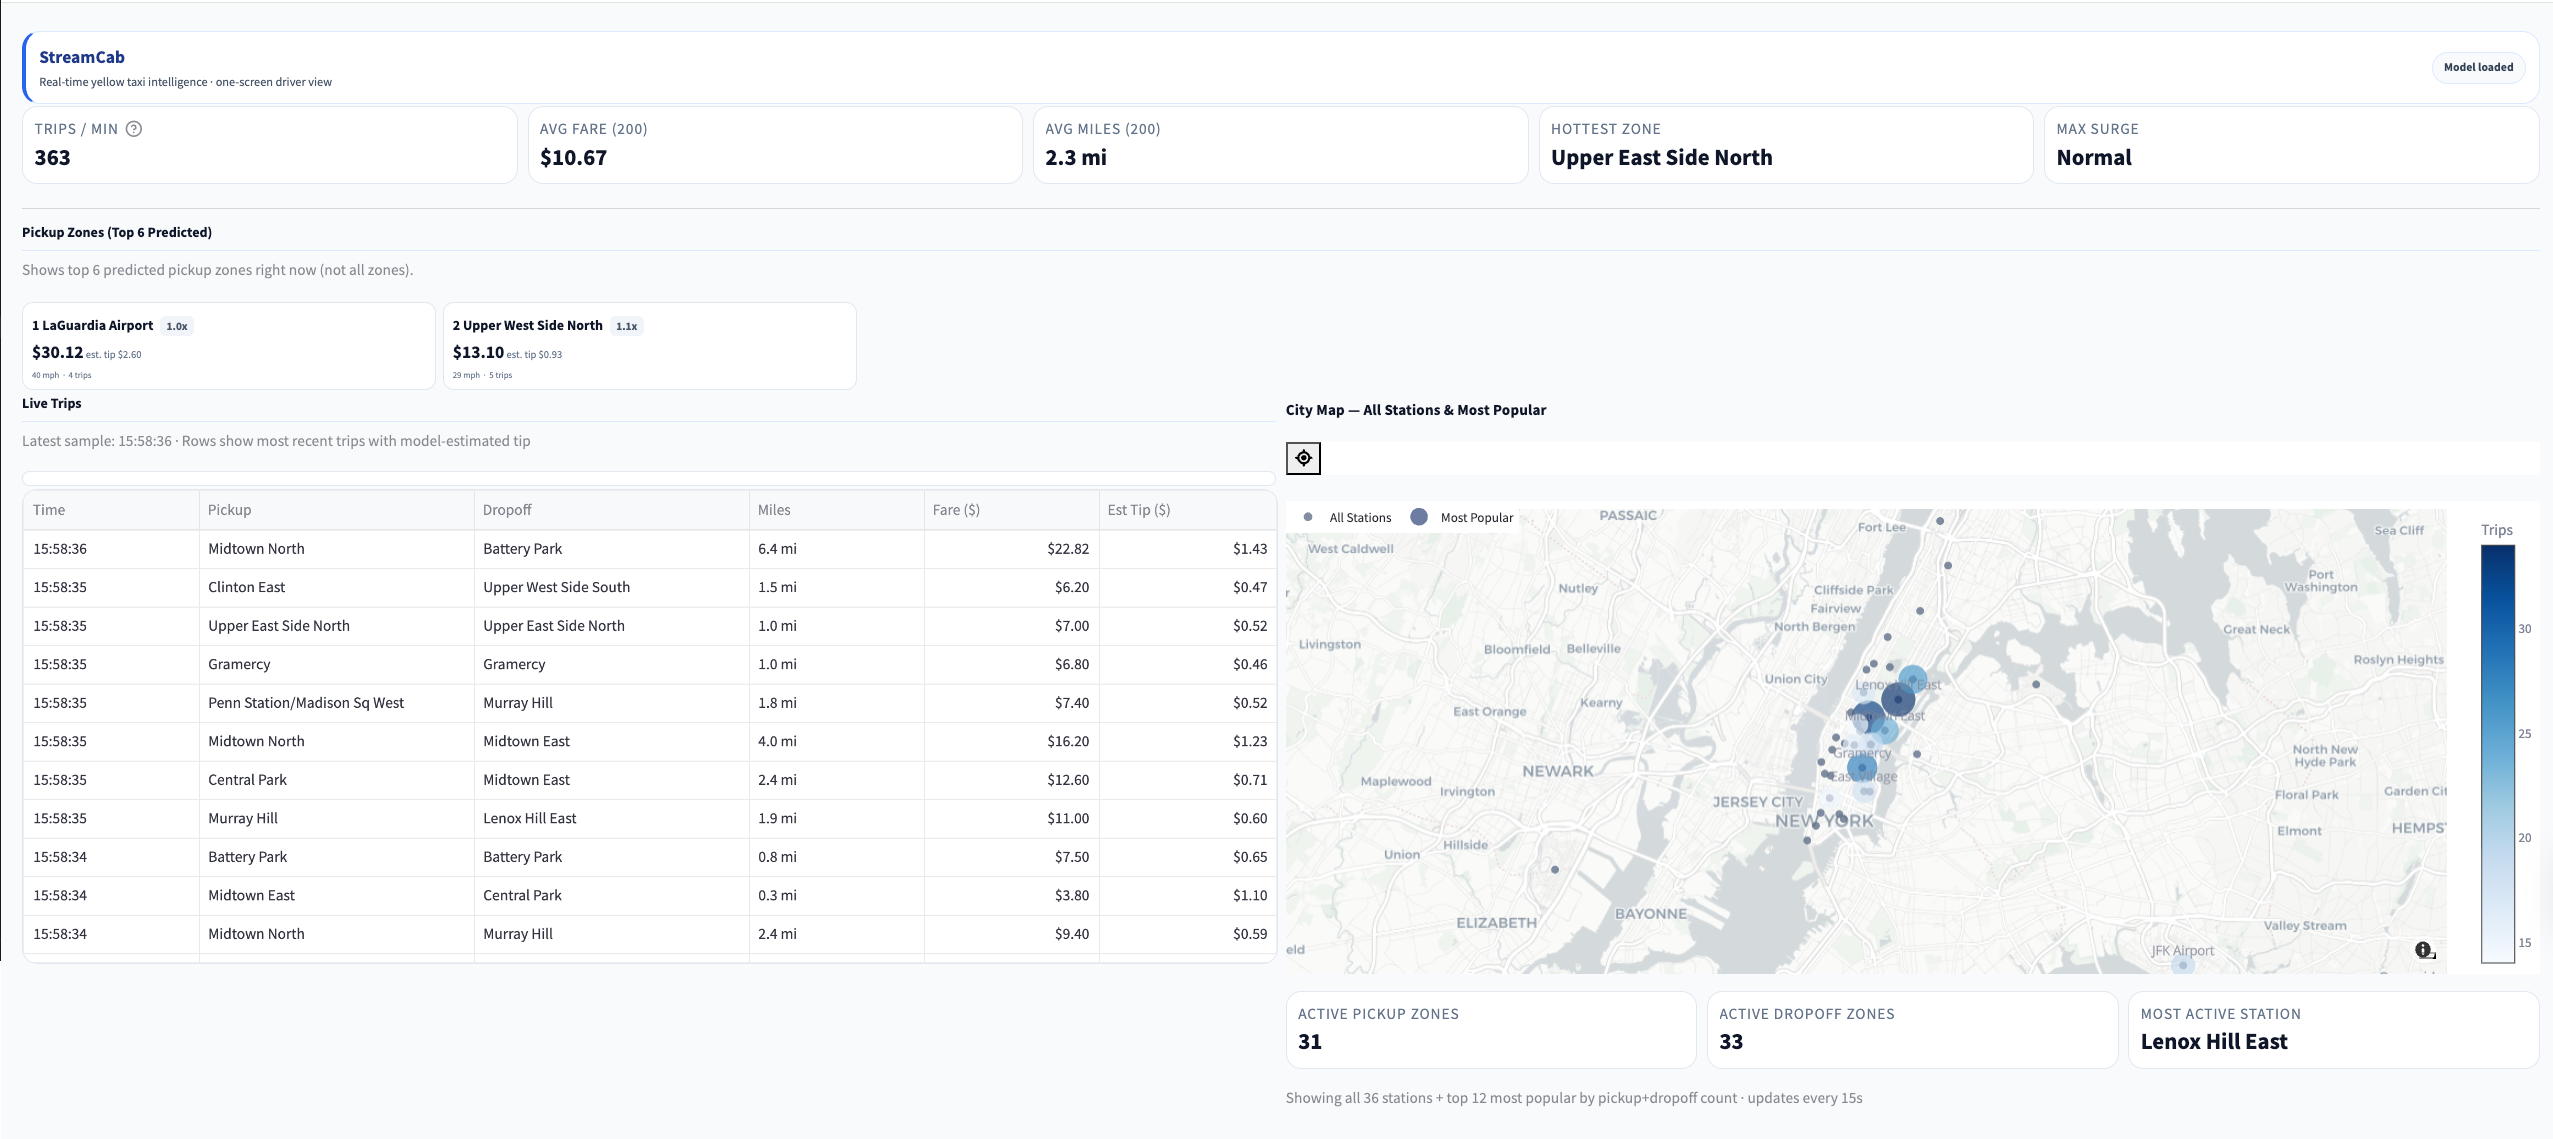
\includegraphics[width=0.95\linewidth]{../assets/app.png}
    \caption{StreamCab dashboard showing live trip table, zone-level insights, and map-based analytics.}\label{fig:dashboard}
\end{figure}

\subsection{Discussion}
The pipeline demonstrates that practical near real-time analytics can be achieved in a local setup when ingestion, processing, and training are designed for bounded memory and idempotent writes. SQL-side narrowing for predictor reads and stream checkpointing significantly improve operational stability.

\subsection{Operational Findings and Reliability Lessons}
Three implementation choices were especially impactful in day-to-day operation:
\begin{itemize}[leftmargin=1.5em]
    \item \textbf{Strict column projection on parquet reads:} lowered I/O and reduced memory pressure during both aggregation and training.
    \item \textbf{Idempotent database writes by time-window keys:} reduced duplicate rows after container restarts.
    \item \textbf{Bounded checkpointed streaming:} improved restart behavior and reduced recomputation cost.
\end{itemize}

In practice, the combination of lightweight observability checks (consumer lag, aggregate freshness, prediction-row sanity) was sufficient to catch most runtime issues before they affected dashboard interpretation.

\subsection{Error Analysis by Scenario}
The largest residual errors were typically observed during abrupt demand-shift windows where historical averages become poor priors. Examples include sudden surges, sparse late-night zones, and transitions between weekday and weekend travel patterns. While aggregate features are stable, they can smooth away micro-context such as weather, event schedules, and incident-driven rerouting.

This suggests two practical extensions: (1) incorporate exogenous signals (weather/events), and (2) support uncertainty-aware outputs (prediction intervals or quantile models) so the dashboard can distinguish confident estimates from high-variance windows.

\subsection{Limitations and Threats to Validity}
Although the quantitative results are strong, several limitations affect generalization and operational confidence. First, the stream is a replay of historical data rather than a true live feed, so observed latency and throughput may differ from production systems with bursty arrival patterns, schema drift, and upstream outages. Second, zone-level aggregates improve model stability but can hide fine-grained effects such as street-level congestion, event-driven anomalies, and rare pickup/dropoff combinations.

The evaluation window is also constrained by selected months and filtering rules. If market conditions shift (fuel prices, policy changes, seasonality, or weather shocks), model error can increase without immediate visibility. Future iterations should include explicit drift indicators (feature distribution shift, residual monitoring, and alarm thresholds) to ensure model performance remains within acceptable bounds. Finally, local single-node deployment simplifies reproducibility, but it does not fully represent fault domains and scaling behavior in distributed environments.

\subsection{Reproducibility and Operational Notes}
To support reproducibility, all services are containerized and orchestrated through Docker Compose with deterministic startup dependencies. The project separates concerns across producer, streaming processor, consumer, trainer, and dashboard services. This isolation reduces coupling and makes it easier to troubleshoot failures by layer. The end-to-end runbook consists of: (1) downloading raw TLC parquet data, (2) launching services, (3) running one-shot training, (4) starting replay/streaming, and (5) validating outputs in PostgreSQL and the dashboard.

Operationally, two implementation choices were especially important. The first is checkpointed stream processing with bounded windows, which limits duplicate writes and supports restart safety. The second is memory-aware training via batched parquet reads and incremental model updates, which enables full-dataset learning on commodity hardware. For teams extending this project, we recommend adding lightweight data quality contracts at ingest time (null/negative checks, timestamp sanity, and schema assertions) and documenting expected service-level objectives for latency and prediction freshness.

The architecture can be extended incrementally: move stateful processing to a managed cluster, introduce model registry/versioning, and add automated backtesting before promoting new models. These steps preserve the current educational value while improving production readiness.

\section{Deployment Trade-Offs and Responsible Use}
\subsection{Scalability Roadmap}
The local-first design was intentional for rapid iteration and reproducibility, but scaling to larger traffic volumes requires architectural adjustments. A practical roadmap is phased: first, externalize state and monitoring; second, separate compute roles; third, harden model lifecycle.

In phase one, the same logical pipeline can run with managed Kafka and managed Postgres while preserving service boundaries. In phase two, Spark processing and model inference should be decoupled so backlog in one stage does not propagate to the other. In phase three, model artifacts should be versioned with promotion gates (offline validation thresholds and rollback hooks). This progression reduces operational risk while keeping the core feature contract intact.

\subsection{Cost and Complexity Considerations}
A key lesson from StreamCab is that reliability improvements are often inexpensive compared to full platform migration. For example, stricter schema checks, idempotent writes, and better observability provide significant stability gains without immediate distributed-cluster overhead.

However, there is a trade-off between implementation simplicity and performance headroom. Small local stacks are easy to reason about and debug, but become brittle under sustained throughput spikes. Distributed deployments improve elasticity but introduce non-trivial complexity in resource tuning, security policy, and incident response. In educational and prototype settings, a staged migration strategy is usually preferable to an immediate all-in rewrite.

\subsection{Data Privacy and Ethical Constraints}
Taxi trip records can reveal sensitive mobility patterns at fine spatial and temporal granularity. Even when identifiers are absent, repeated trajectories may indirectly expose behavioral signals. For this reason, outputs should prioritize aggregate reporting over row-level redistribution, and access to raw tables should follow least-privilege principles.

Model predictions should also be interpreted as decision support rather than ground truth. Overconfident use in operational dispatch or pricing may amplify existing geographic inequities if data coverage differs by zone. Recommended safeguards include confidence annotation, periodic bias checks across zones/time windows, and human review for high-impact policy decisions.

These constraints do not prevent practical use; they define guardrails for responsible deployment. Incorporating governance from the start generally improves long-term trust and reduces rework in later productionization stages.

\section{Conclusion and Key Takeaways}
\textbf{What worked well:}
\begin{itemize}[leftmargin=1.5em]
    \item Modular services and reproducible local orchestration.
    \item Streaming aggregates as robust prediction features.
    \item Strong tabular prediction performance with XGBoost.
\end{itemize}

\textbf{Main challenges:}
\begin{itemize}[leftmargin=1.5em]
    \item Large data volume vs local memory constraints.
    \item Reliability semantics across stream and database boundaries.
    \item Balancing latency, correctness, and simplicity.
\end{itemize}

\textbf{Future work:}
\begin{itemize}[leftmargin=1.5em]
    \item Add drift monitoring and automated retraining schedules.
    \item Extend features with weather/events/geospatial context.
    \item Compare distributed multi-node deployment variants.
\end{itemize}


\begin{thebibliography}{9}
\bibitem{tlc}
NYC Taxi \& Limousine Commission,
\textit{TLC Trip Record Data},
\url{https://www.nyc.gov/site/tlc/about/tlc-trip-record-data.page}

\bibitem{kafka}
Apache Kafka Documentation,
\url{https://kafka.apache.org/documentation/}

\bibitem{spark}
Apache Spark Structured Streaming Guide,
\url{https://spark.apache.org/docs/latest/structured-streaming-programming-guide.html}

\bibitem{xgboost}
T. Chen and C. Guestrin,
\textit{XGBoost: A Scalable Tree Boosting System}, KDD 2016.
\end{thebibliography}

\end{document}
